% !TEX TS-program = pdflatexmk
\documentclass[12pt]{article}

% Layout.
\usepackage[top=1in, bottom=0.75in, left=1in, right=1in, headheight=1in, headsep=6pt]{geometry}

% Fonts.
\usepackage{mathptmx}
\usepackage[scaled=0.86]{helvet}
\renewcommand{\emph}[1]{\textsf{\textbf{#1}}}
\newcommand{\ans}[1][1in]{\rule{#1}{.5pt}}

\usepackage[parfill]{parskip}
\usepackage{adjustbox}

% Misc packages.
\usepackage{amsmath,amssymb,latexsym}
\usepackage{graphicx,hyperref}
\usepackage{array}
\usepackage{xcolor}
\usepackage{multicol,tikz}
\usepackage{tabularx,colortbl,booktabs,xparse}
\usepackage{enumitem}

\renewcommand{\familydefault}{\sfdefault}

\usetikzlibrary{calc,trees,positioning,arrows,fit,shapes,through, backgrounds}
\usetikzlibrary{patterns}


\NewDocumentCommand{\rot}{O{45} O{1em} m}{\makebox[#2][l]{\rotatebox{#1}{#3}}}%

\usepackage{fancyhdr}
\pagestyle{fancy} 
\lhead{\large\sf\textbf{MATH F113X: Introduction to Scheduling}}
%\chead{}
%\rhead{}

\begin{document}
\textbf{Goal} Learn about the following terminology: schedule, digraph, processors, finishing time, optimal finishing time, optimal schedule, idle time, critical path, critical time.\\

\begin{enumerate}
\item \textbf{Motivating Example} Fixing a Flat Bike Tire\\

\begin{tabular}{llll}
label&task&time&dependence\\
\hline
A&buy a replacement tube&20 minutes&\\
&patch kit&&\\
B&find tools&5 minutes&\\
C&remove tire and tube&10 minutes&\\
D&replace tire and new tube&10 minutes&\\
E&repair old tube&10 minutes&\\
\end{tabular}
\vfill
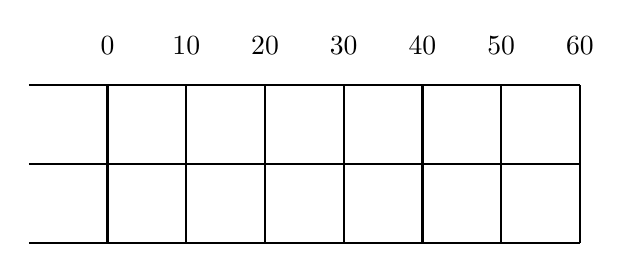
\begin{tikzpicture}
\foreach \x [evaluate=\x as \xeval using int(\x*10)] in {0,1,...,6}{
	\node  at (\x,2.5){$\xeval$};
	\draw[thick] (\x,0) -- (\x,2);
	}
\foreach \y in {0,1,2}{\draw[thick] (-1,\y)--(6,\y);}
\end{tikzpicture}
\vspace{.3in}

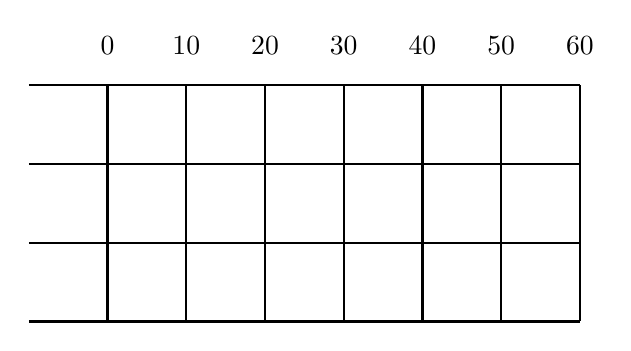
\begin{tikzpicture}
\foreach \x [evaluate=\x as \xeval using int(\x*10)] in {0,1,...,6}{
	\node  at (\x,3.5){$\xeval$};
	\draw[thick] (\x,0) -- (\x,3);
	}
\foreach \y in {0,1,2,3}{\draw[thick] (-1,\y)--(6,\y);}
\end{tikzpicture}
\newpage
\item Terminology
	\begin{enumerate}
	\item \textbf{schedule}
	\vfill
	\item \textbf{digraph}
	\vfill
	\item \textbf{processors}
	\vfill
	\item \textbf{finishing time}
	\vfill
	\item \textbf{optimal finishing time and optimal schedule}
	\vfill
	\item \textbf{idle time}
	\vfill
	\item \textbf{critical path}
	\vfill
	\item \textbf{critical time}
	\vfill
	\end{enumerate}

\item \textbf{General Example}: Create a digraph. Make a valid schedule with TWO processors. Determine values of finishing time, idle time and critical time.\\

\begin{tabular}{llll}
label/task&time&dependence\\
\hline
A&2&\\
B&1&\\
C&2&\\
D&3&A\\
E&6&A,B\\
F&8&B,C\\
G&5&E,F\\
\end{tabular}


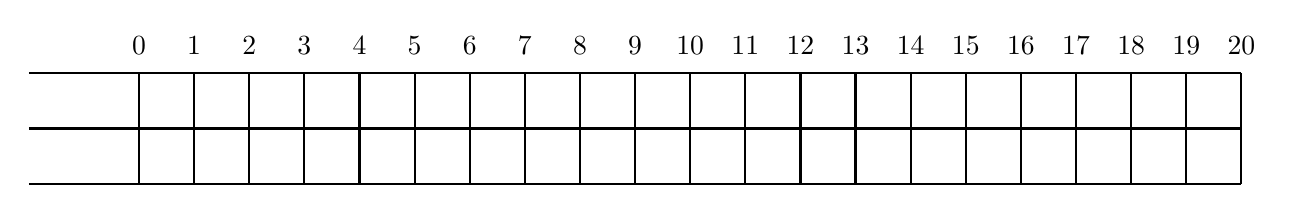
\begin{tikzpicture}[scale=.7]
\foreach \x in {0,1,...,20}{
	\node  at (\x,2.5){$\x$};
	\draw[thick] (\x,0) -- (\x,2);
	}
\foreach \y in {0,1,2}{\draw[thick] (-2,\y)--(20,\y);}
\end{tikzpicture}
\end{enumerate}
\end{document}